%%%%%%%%%%%%%%%%%%%%%%%%%%%%%%%%%%%%%%%%%
% baposter portrait poster - Single-pixel camera + 3D Gaussian Splatting (Truck scene)
% All numbers come from results/*.csv of the spc-gs repository. Figures are in figs_spc/.
%%%%%%%%%%%%%%%%%%%%%%%%%%%%%%%%%%%%%%%%%
\documentclass[portrait,paperwidth=800mm,paperheight=1000mm,fontscale=0.37]{baposter}
\usepackage{graphicx}
\graphicspath{{figs_spc/}{figures/}}
\usepackage{tabularx}
\usepackage[most]{tcolorbox}
\usepackage{amsmath}
\usepackage{amssymb}
\usepackage{booktabs}
\usepackage{adjustbox}
\usepackage{enumitem}
\usepackage{palatino}
\usepackage{qrcode}
\usepackage{pgf,tikz}
\usetikzlibrary{arrows.meta,shapes,positioning,calc}


\newcommand{\compresslist}{%
\setlength{\itemsep}{0.6ex}\setlength{\parskip}{0pt}\setlength{\parsep}{0pt}\setlength{\topsep}{0.3ex}}
\definecolor{usmblue}{RGB}{0,62,133}
\definecolor{lightblue}{rgb}{0.145,0.6666,1}
\definecolor{accent}{RGB}{217,95,2}
% Uniform figure caption
\newcommand{\figcap}[1]{\par\smallskip{\small\itshape #1}\par}
% Key-number card: big value + label (fixed height, identical style)
\newcommand{\card}[3]{%
 \begin{tcolorbox}[enhanced,colback=lightblue!12,colframe=#3,boxrule=1.2pt,arc=3mm,%
   left=2mm,right=2mm,top=2mm,bottom=2mm,height=4.9em,valign=center,halign=center]
 {\LARGE\bfseries\color{#3}#1}\par\smallskip{\small #2}%
 \end{tcolorbox}}
% Highlight box
\newenvironment{callout}[1][usmblue]{\begin{tcolorbox}[enhanced,colback=#1!8,colframe=#1,boxrule=1.2pt,arc=2mm,left=2mm,right=2mm,top=1mm,bottom=1mm]}{\end{tcolorbox}}

\begin{document}
\begin{poster}
{
headerborder=closed,
colspacing=0.6em,
bgColorOne=white,
bgColorTwo=white,
borderColor=usmblue,
headerColorOne=usmblue,
headerColorTwo=usmblue,
headerFontColor=white,
boxColorOne=white,
textborder=roundedleft,
eyecatcher=true,
headerheight=0.082\textheight,
headershape=roundedright,
headerfont=\Large\bf\textsc,
linewidth=2pt
}
%----------------------------------------------------------------------------------------
{
\includegraphics[height=4.5em]{WACCI_logo.png}}
{\bf\textsc{\Large{How many measurements does a single-pixel camera need?}}\\[0.3ex]
 \textsc{\large From 2D reconstruction to 3D Gaussian Splatting}\vspace{0.1cm}}
{\textsc{
    \large{Francisco Alfaro$^1$ and Ayrton Perez$^2$}\\
    \small{
        $^1$Department of Electronics \quad
        $^2$Department of Informatics\\
        Universidad T\'ecnica Federico Santa Mar\'ia, Chile\\
        \textcolor{blue}{francisco.alfaro@usm.cl, ayrton.perez@usm.cl}
    }
}}
{
\includegraphics[height=6.0em]{usm.png}}

%----------------------------------------------------------------------------------------
%----------------------------------------------------------------------------------------
\headerbox{Motivation and question}{name=motiv,column=0,row=0}{
\raggedright
A \textbf{single-pixel camera (SPC)} replaces the sensor matrix by one photodetector and a sequence of coded patterns:
a simpler sensor, but \textbf{more measurements per image}. For 3D scenes the cost multiplies, because 3D Gaussian
Splatting (3DGS) needs many views.
\smallskip

\begin{callout}[accent]
\textbf{Question.} How much quality is lost in the 2D views, and in the 3D model trained on them, when only
5, 10, 25 or 50\,\% of the measurements are taken? Does the pattern (Hadamard, random, DCT) or the reconstruction
(direct, TV) change the answer?
\end{callout}
}

%----------------------------------------------------------------------------------------
\headerbox{Single-pixel camera}{name=model,column=0,below=motiv}{
\raggedright
\centering
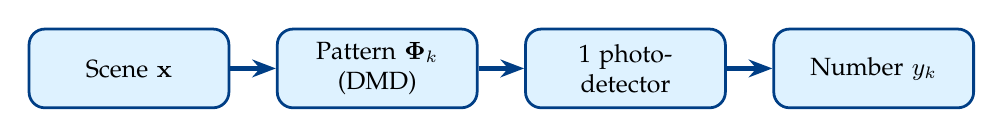
\begin{tikzpicture}[x=\linewidth, nodo/.style={draw=usmblue,fill=lightblue!15,rounded corners=2mm,line width=1pt,minimum height=10mm,
  text width=0.19\linewidth,align=center,font=\small}, flecha/.style={-{Stealth[length=3mm]},line width=1.6pt,usmblue}]
 \node[nodo] (a) at (0.11,0) {Scene $\mathbf{x}$};
 \node[nodo] (b) at (0.37,0) {Pattern $\mathbf{\Phi}_k$ (DMD)};
 \node[nodo] (c) at (0.63,0) {1 photo-detector};
 \node[nodo] (d) at (0.89,0) {Number $y_k$};
 \draw[flecha] (a)--(b); \draw[flecha] (b)--(c); \draw[flecha] (c)--(d);
\end{tikzpicture}
\raggedright\smallskip

\textbf{One measurement} = the light that passes through one pattern: multiply scene and pattern pixel by pixel and add (an inner product). Many patterns give:
\vspace{-0.5ex}
\[
\mathbf{y}=\mathbf{\Phi}\mathbf{x}+\mathbf{n},\qquad \mathbf{\Phi}\in\mathbb{R}^{K\times N}
\]
\vspace{-1.5ex}
\begin{itemize}\compresslist
 \item $N$ = pixels, $K$ = patterns. The \textbf{ratio} $r=K/N$ is the fraction of the image that is measured: smaller $r$ is faster, but harder to reconstruct.
 \item Rows of $\mathbf{\Phi}$ are orthonormal ($\mathbf{\Phi}\mathbf{\Phi}^{\top}=\mathbf{I}$) and applied with fast transforms, so $\mathbf{\Phi}$ is never stored.
\end{itemize}
}

%----------------------------------------------------------------------------------------
\headerbox{Patterns and reconstruction}{name=patrones,column=0,below=model}{
\raggedright
\centering
\adjustbox{trim=0 {0.14\height} 0 0,clip,width=0.92\linewidth}{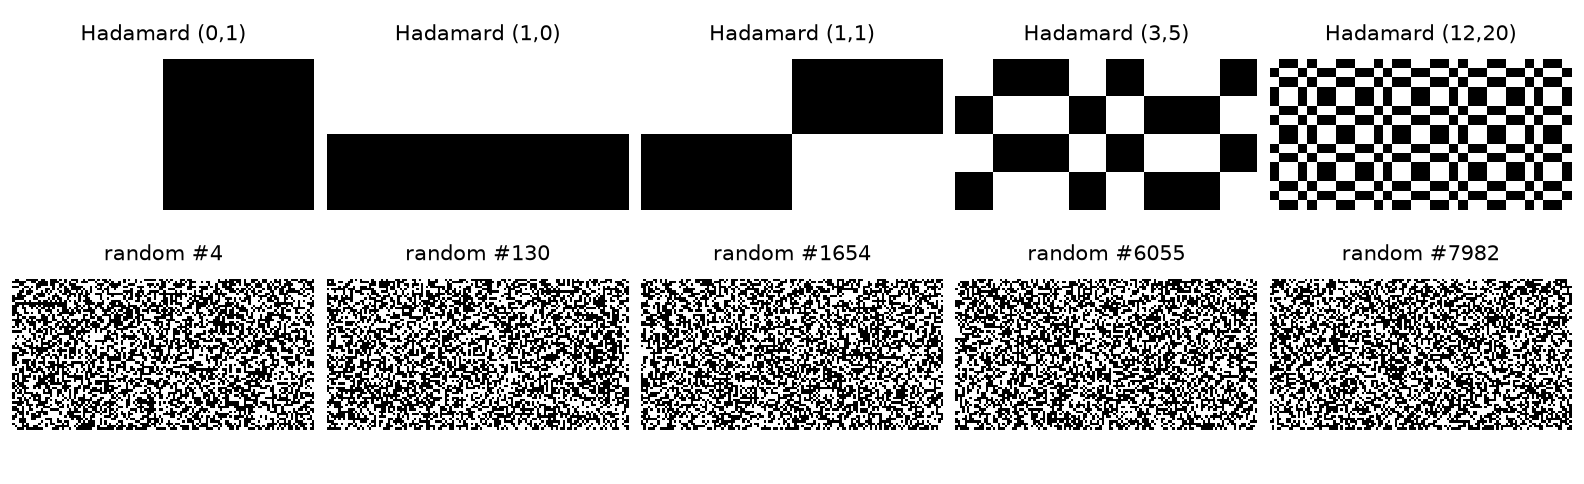
\includegraphics{fig_patterns.png}}
\figcap{Hadamard (ordered by sequency) and random binary patterns.}
\raggedright
\begin{itemize}\compresslist
 \item \textbf{Hadamard:} black/white, coarse to fine (low frequencies first). \textbf{Random:} permuted Hadamard, DC always measured. \textbf{DCT:} smooth cosines, reference (not binary).
 \item \textbf{Direct:} one fast product $\hat{\mathbf{x}}=\mathbf{\Phi}^{\top}\mathbf{y}$, no image prior.
 \item \textbf{TV (FISTA):} keep, among the images that fit the data, the most piecewise smooth:
\end{itemize}
\vspace{-1ex}
\[
\hat{\mathbf{x}}=\arg\min_{\mathbf{x}}\ \tfrac12\|\mathbf{\Phi x}-\mathbf{y}\|_2^2+\lambda\,\mathrm{TV}(\mathbf{x}),\ \ \lambda=0.003
\]
}

%----------------------------------------------------------------------------------------
%----------------------------------------------------------------------------------------
%----------------------------------------------------------------------------------------
\headerbox{What is 3D Gaussian Splatting?}{name=gs,column=1,span=2,row=0}{
\raggedright
\begin{minipage}[t]{0.44\linewidth}\vspace{0pt}\centering
\adjustbox{trim={0.05\width} {0.03\height} {0.05\width} {0.06\height},clip,width=\linewidth}{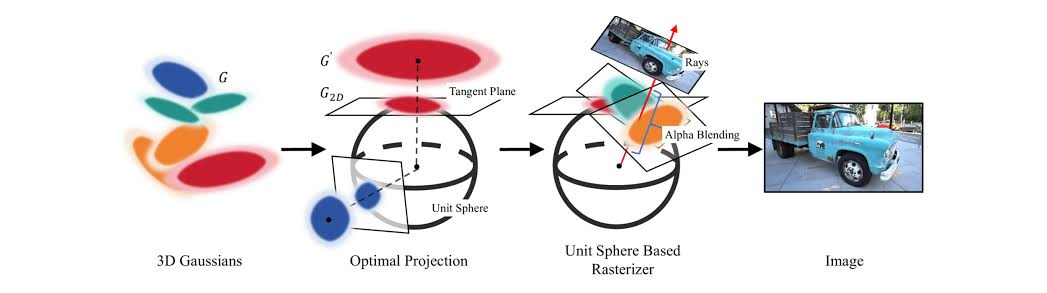
\includegraphics{gs.jpeg}}
\figcap{3DGS rendering: 3D Gaussians are projected and alpha-blended into an image. Figure: SOURCE TO BE CONFIRMED.}
\end{minipage}\hfill
\begin{minipage}[t]{0.53\linewidth}\vspace{0pt}\raggedright
\begin{enumerate}[leftmargin=*,label=\textbf{\arabic*.}]\compresslist
 \item \textbf{Represent:} the scene is a cloud of millions of 3D Gaussians, each with a position, a covariance (shape), an opacity and a color.
 \item \textbf{Splat:} each Gaussian is projected onto the image plane and the overlapping ones are alpha-composited, front to back.
 \item \textbf{Optimize:} gradient descent compares the render with the training views (photometric loss); Gaussians are split, cloned or pruned adaptively.
 \item \textbf{Why many views:} every view constrains the 3D geometry; this is why reducing the measurements \emph{per view} matters.
\end{enumerate}
\end{minipage}
}

%----------------------------------------------------------------------------------------
\headerbox{Experimental pipeline}{name=metodos,column=1,span=2,below=gs}{
\raggedright
\centering
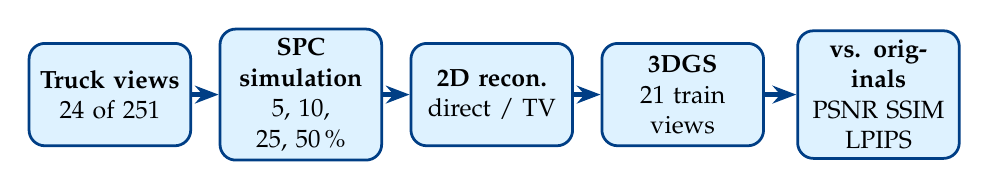
\begin{tikzpicture}[x=\linewidth,y=1mm,
  nodo/.style={draw=usmblue,fill=lightblue!15,rounded corners=2mm,line width=1pt,
    minimum width=0.165\linewidth,text width=0.15\linewidth,minimum height=13mm,align=center,font=\small},
  flecha/.style={-{Stealth[length=3mm]},line width=1.8pt,usmblue}]
 \node[nodo] (a) at (0.085,0)  {\textbf{Truck views}\\24 of 251};
 \node[nodo] (b) at (0.285,0) {\textbf{SPC simulation}\\5, 10, 25, 50\,\%};
 \node[nodo] (c) at (0.485,0)  {\textbf{2D recon.}\\direct / TV};
 \node[nodo] (d) at (0.685,0) {\textbf{3DGS}\\21 train views};
 \node[nodo] (e) at (0.89,0)  {\textbf{vs. originals}\\PSNR SSIM LPIPS};
 \draw[flecha] (a.east)--(b.west); \draw[flecha] (b.east)--(c.west);
 \draw[flecha] (c.east)--(d.west); \draw[flecha] (d.east)--(e.west);
\end{tikzpicture}
\smallskip

\raggedright
\begin{minipage}[t]{0.49\linewidth}\vspace{0pt}\raggedright
\begin{itemize}\compresslist
 \item \textbf{Scene:} Truck (Tanks and Temples), 979$\times$546; 3 test views, 21 training views, 230 held-out views.
 \item \textbf{Grids:} 256$\times$512 (25\,\% of the pixels) and 512$\times$1024 (98\,\%).
\end{itemize}
\end{minipage}\hfill
\begin{minipage}[t]{0.49\linewidth}\vspace{0pt}\raggedright
\begin{itemize}\compresslist
 \item \textbf{Control:} resample to the grid and back, no SPC. \textbf{Baseline:} 3DGS on original images.
 \item \textbf{Metrics} always against the \emph{original} images, full resolution.
\end{itemize}
\end{minipage}
}

%----------------------------------------------------------------------------------------
\headerbox{2D results: SPC reconstruction}{name=res2d,column=1,span=2,below=metodos}{
\raggedright
\centering
\adjustbox{trim=0 {0.12\height} 0 0,clip,width=\linewidth}{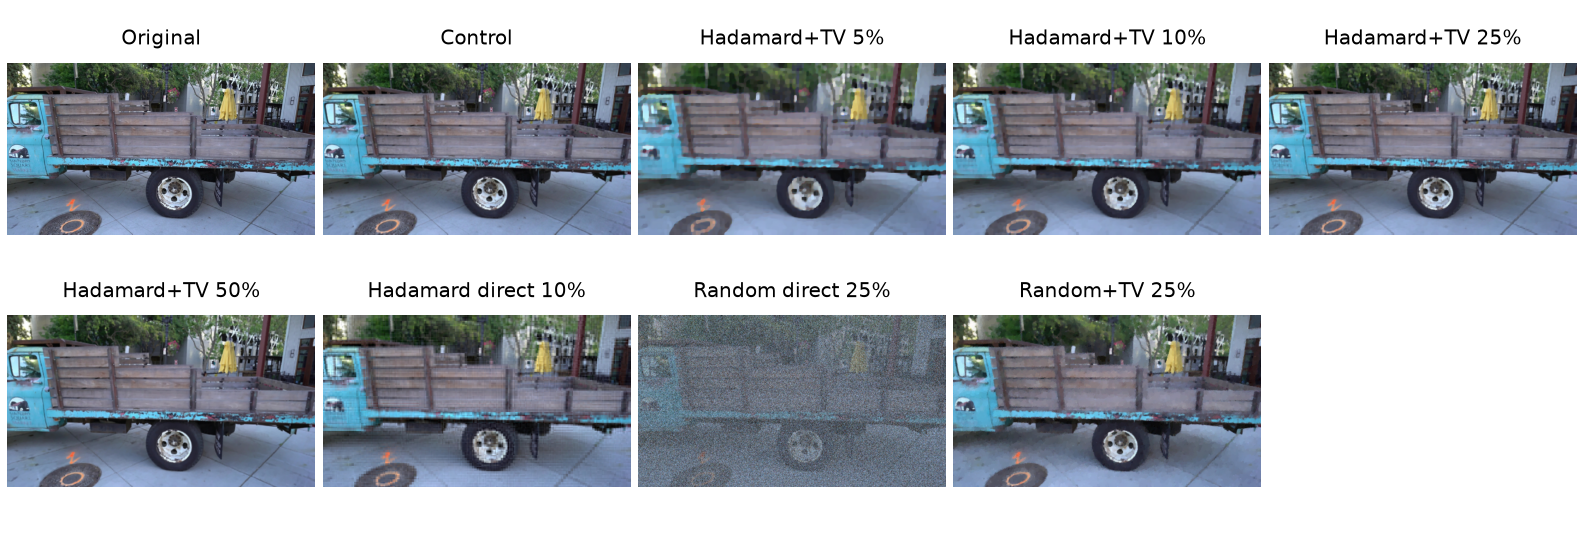
\includegraphics{fig_2d_visual.png}}
\figcap{Training view 000208. TV recovers the slats and wheel from 25\,\%.}
\medskip

\raggedright
\begin{minipage}[t]{0.50\linewidth}\vspace{0pt}\raggedright
\textbf{PSNR (dB)}, grid 256$\times$512, 24 views
\smallskip

\small
\renewcommand{\arraystretch}{1.05}
\begin{tabular*}{\linewidth}{@{}l@{\extracolsep{0pt plus 1fill}}cccc@{}}
\toprule
Pattern, method & 5\,\% & 10\,\% & 25\,\% & 50\,\% \\
\midrule
Hadamard, direct  & 20.63 & 21.89 & 23.92 & 25.92 \\
Hadamard, TV      & 21.52 & 22.89 & 24.87 & 26.33 \\
Random, direct & 12.65 & 12.93 & 13.87 & 15.82 \\
Random, TV      & 20.35 & 21.89 & 24.39 & 26.12 \\
DCT, TV      & \textbf{21.80} & \textbf{23.18} & \textbf{25.17} & \textbf{26.49} \\
\midrule
Control (no SPC) & \multicolumn{4}{c}{27.22} \\
\bottomrule
\end{tabular*}
\end{minipage}\hfill
\begin{minipage}[t]{0.47\linewidth}\vspace{0pt}\raggedright
\begin{itemize}\compresslist
 \item Loss vs. control with Hadamard + TV: \textbf{5.70, 4.33, 2.35, 0.89\,dB}.
 \item TV adds 0.4 to 1.0\,dB over direct.
 \item Random needs TV: direct fails (12.7 to 15.8\,dB).
\end{itemize}
\end{minipage}
}

%----------------------------------------------------------------------------------------
\headerbox{3D results (3DGS, 7000 iterations)}{name=res3d,column=1,span=2,below=res2d}{
\raggedright
\begin{minipage}[t]{0.315\linewidth}\vspace{0pt}\card{19.38 dB}{Held-out PSNR, Hadamard + TV 50\,\% (baseline 19.40)}{usmblue}\end{minipage}\hfill
\begin{minipage}[t]{0.315\linewidth}\vspace{0pt}\card{$\approx$ 2D}{Training views inherit the 2D loss (25.90 vs. 26.33 dB at 50\,\%)}{accent}\end{minipage}\hfill
\begin{minipage}[t]{0.315\linewidth}\vspace{0pt}\card{3 views}{Test PSNR is not conclusive: 17 of 42 pairs}{usmblue}\end{minipage}

\smallskip
\centering
\adjustbox{trim=0 {0.015\height} 0 {0.07\height},clip,width=\linewidth}{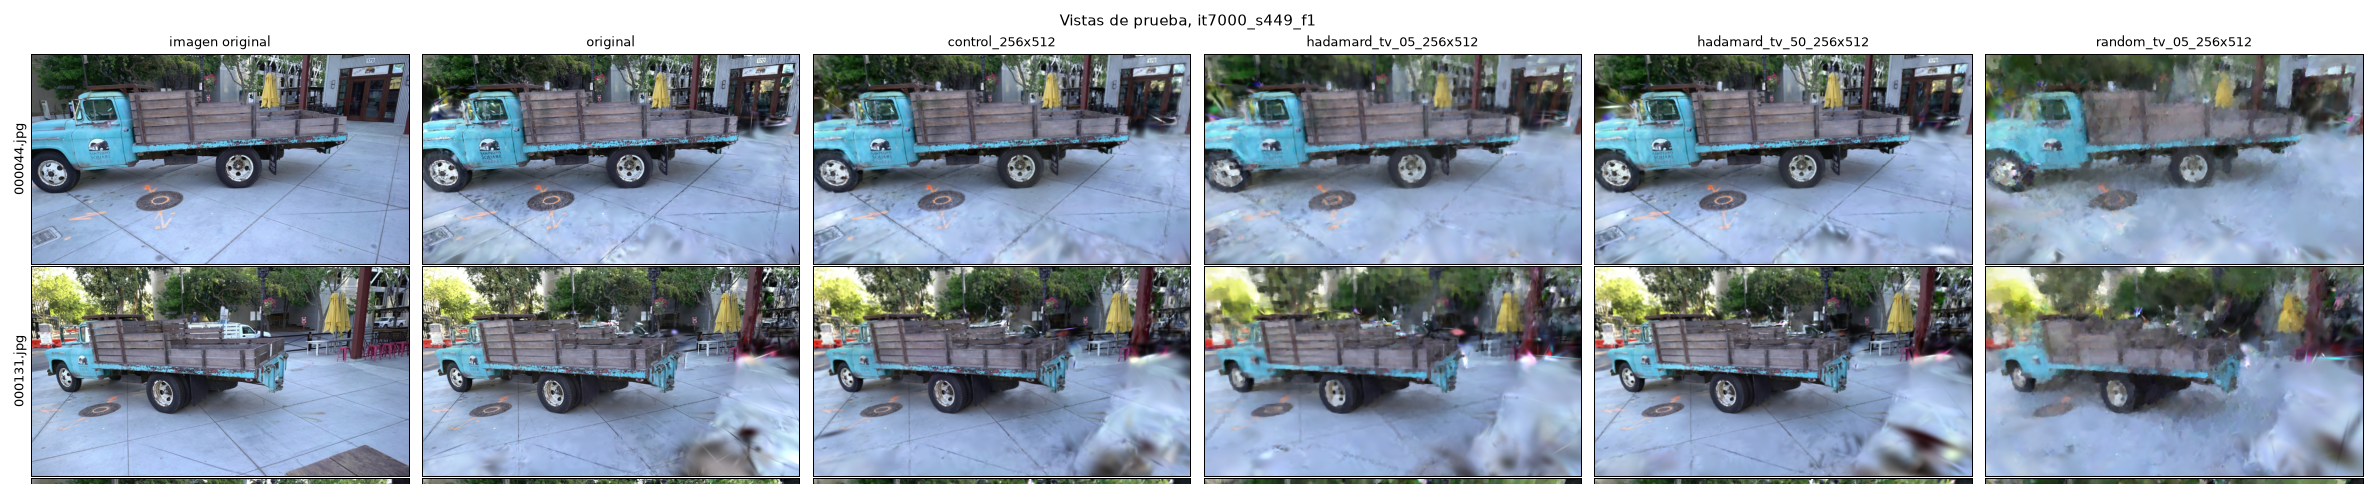
\includegraphics{fig_3d_renders.png}}
\figcap{Test views 000044 and 000131 (columns: original image, baseline, control, Hadamard + TV 5\,\% and 50\,\%, random + TV 5\,\%).}
}

%----------------------------------------------------------------------------------------
\headerbox{Computational cost}{name=costo,column=0,below=patrones}{
\raggedright
\small
\renewcommand{\arraystretch}{1.0}
\begin{tabular*}{\linewidth}{@{}l@{\extracolsep{0pt plus 1fill}}r@{}}
\toprule
Stage & Time \\
\midrule
2D direct & $\le$ 7 ms / view \\
2D TV, 256$\times$512 & 0.99--1.27 s / view \\
2D TV, 512$\times$1024 & 1.69--1.75 s / view \\
3DGS 3000 / 7000 it. & 63--90 s / 146--384 s \\
3DGS 30\,000 it. & 1140--3495 s \\
\bottomrule
\end{tabular*}
\par\smallskip
Peak memory 1.0--6.3\,GiB (SPC).
\par\smallskip
\textbf{Hardware:} RTX 4060 Laptop (8\,GB), WSL2 Ubuntu 24.04, CUDA 12.8, gsplat 1.5.3. Seed 449. Noise off in the main results. Baseline check (251 views): 23.54 dB vs. 23.51 dB published.
}

%----------------------------------------------------------------------------------------
\headerbox{Conclusions and limits}{name=concl,column=1,span=2,below=res3d,above=bottom}{
\raggedright
\begin{minipage}[t]{0.49\linewidth}\vspace{0pt}\raggedright
\begin{itemize}\compresslist
 \item \textbf{2D:} Hadamard + TV loses 0.89\,dB at 50\,\% and 5.70\,dB at 5\,\% vs. the control.
 \item \textbf{3D:} inherits the 2D loss up to $\approx$28.5\,dB, then saturates (31--32\,dB). On 230 held-out views, 50\,\% matches the baseline (10\,\% on the 512$\times$1024 grid).
\end{itemize}
\end{minipage}\hfill
\begin{minipage}[t]{0.49\linewidth}\vspace{0pt}\raggedright
\begin{itemize}\compresslist
 \item \textbf{Limits:} one scene, one seed, COLMAP poses from original images (optimistic), simulated optics.
 \item \textbf{Next:} more scenes, re-estimated poses, 3DGS from the measurements.
\end{itemize}
\end{minipage}
}

%----------------------------------------------------------------------------------------
\headerbox{Code and references}{name=refs,column=0,below=costo,above=bottom}{
\raggedright
\begin{minipage}[c]{0.17\linewidth}\centering
\qrcode[height=\linewidth]{https://github.com/fralfaro/spc-gs}
\end{minipage}\hfill
\begin{minipage}[c]{0.78\linewidth}\raggedright\small
\textbf{Open source:}\\ github.com/fralfaro/spc-gs\\
Configs, tests and all CSV files.
\end{minipage}

\vspace{1ex}
\footnotesize
\setlength{\parskip}{0pt}
\noindent [1] Duarte et al., IEEE Signal Process. Mag., 2008.\par
\noindent [2] Yu et al., \textit{cake-cutting}, Sensors, 2019.\par
\noindent [3] Rudin et al., Physica D, 1992.\par
\noindent [4] Beck and Teboulle, SIAM J. Imaging Sci., 2009.\par
\noindent [5] Kerbl et al., ACM TOG, 2023.\par
\noindent [6] Ye et al., gsplat, arXiv:2409.06765, 2024.\par
\noindent [7] Knapitsch et al., ACM TOG, 2017.
}

\end{poster}
\end{document}
